\documentclass[11pt]{amsart}
\usepackage{amsmath,amssymb,amsthm,mathtools}
\usepackage[margin=1in]{geometry}
\usepackage{hyperref}
\usepackage{graphicx}
\graphicspath{{./}{../figures/}}

\newtheorem{proposition}{Proposition}
\newtheorem{corollary}[proposition]{Corollary}
\theoremstyle{remark}
\newtheorem{remark}[proposition]{Remark}
\newtheorem*{example}{Example}

\title{Area Distortion and Exact Band Geometry of the AM--GM Cone}
\author{Jeremy Ebert}
\address{Franklin County, Ohio, USA}
\date{2026}

\begin{document}
\maketitle

\begin{abstract}
For the mean-value coordinates
\[
X=\frac{x-y}{2},\qquad Y=\sqrt{xy},\qquad T=\frac{x+y}{2},
\]
which satisfy $X^2+Y^2=T^2$, we derive the exact area distortion from the positive factor plane to the flat $(X,Y)$ circle view and then to the induced Euclidean area on the cone. The flat Jacobian is
\[
dX\,dY=\frac{x+y}{4\sqrt{xy}}\,dx\,dy=\frac{T}{2Y}\,dx\,dy,
\]
while cone surface area is exactly $\sqrt2$ times flat-shadow area. Anti-diagonal triangles map to half-disks with global unweighted area ratio $\pi/4$, constant-product hyperbolas $xy=n$ map to horizontal secants $Y=\sqrt n$, and the resulting hyperbola/secant partition admits closed formulas on both sides of the map. In logarithmic factor-ratio coordinates, the transformation compactifies the rapidity variable $s=\tfrac12\log(x/y)$ into the ordinary circle angle $\theta$ by
\[
\sin\theta=\tanh s,\qquad \cos\theta=\operatorname{sech}s,\qquad d\theta=\operatorname{sech}s\,ds.
\]
Most importantly, the original factor-plane measure is recovered in circle coordinates by the exact weighted measure
\[
dx\,dy=2\cos\theta\,dX\,dY=2\operatorname{sech}s\,dX\,dY.
\]
Thus the logarithmic, circular, and area descriptions are connected by an exact change of variables rather than by a constant area-preserving identification.
\end{abstract}

\section{The factor-plane map}
For $x,y>0$ define
\begin{equation}
X=\frac{x-y}{2},\qquad Y=\sqrt{xy},\qquad T=\frac{x+y}{2}. \tag{1}
\end{equation}
Then
\begin{equation}
X^2+Y^2=T^2,\qquad x=T+X,\qquad y=T-X. \tag{2}
\end{equation}
The map
\[
F:(x,y)\longmapsto(X,Y)
\]
is a diffeomorphism from the open positive quadrant onto the open upper half-plane $Y>0$.

\begin{proposition}[Exact flat-area Jacobian]\label{prop:flatjac}
The factor-plane area element and flat circle-view area element are related by
\begin{equation}
\boxed{
 dX\,dY=\frac{x+y}{4\sqrt{xy}}\,dx\,dy
 =\frac{T}{2Y}\,dx\,dy.}
\tag{3}
\end{equation}
\end{proposition}

\begin{proof}
From (1),
\[
X_x=\frac12,\quad X_y=-\frac12,\quad
Y_x=\frac12\sqrt{\frac yx},\quad
Y_y=\frac12\sqrt{\frac xy}.
\]
Hence
\[
\left|\frac{\partial(X,Y)}{\partial(x,y)}\right|
=\frac14\left(\sqrt{\frac xy}+\sqrt{\frac yx}\right)
=\frac{x+y}{4\sqrt{xy}}
=\frac{T}{2Y}.
\]
\end{proof}

\begin{remark}
The distortion is not constant. It is smallest on the diagonal $x=y$, where it equals $1/2$, and diverges toward either factor axis. This is the precise obstruction to identifying ordinary multiplication-table area directly with Euclidean area in the circle view.
\end{remark}

\section{From the circle view to the cone surface}
The cone is the graph $T=\sqrt{X^2+Y^2}$ over the upper half-plane. Away from the apex,
\[
|\nabla T|^2=1,
\]
so its Euclidean surface element is
\begin{equation}
\boxed{dA_{\rm cone}=\sqrt2\,dX\,dY.}\tag{4}
\end{equation}
Combining (3) and (4) gives
\begin{equation}
\boxed{
 dA_{\rm cone}=\frac{x+y}{2\sqrt2\sqrt{xy}}\,dx\,dy
 =\frac{T}{\sqrt2\,Y}\,dx\,dy.}
\tag{5}
\end{equation}
This is the induced-area formula derived independently in the earlier semiclassical note; here it is used purely geometrically.

\begin{proposition}[Exact anti-diagonal band area]\label{prop:band}
The factor strip
\[
K\le x+y\le K+2
\]
maps to the half-annulus with radii $T_1=K/2$ and $T_2=(K+2)/2$. Its flat-shadow area is
\begin{equation}
A_{\rm shadow}(K)=\frac\pi2(T_2^2-T_1^2)=\frac\pi2(K+1), \tag{6}
\end{equation}
and its induced cone-surface area is
\begin{equation}
\boxed{A_{\rm band}(K)=\frac\pi{\sqrt2}(K+1).}\tag{7}
\end{equation}
\end{proposition}

\section{Whole triangles map to half-disks}
For $S>0$ let
\[
\Delta_S=\{(x,y):x\ge0,\ y\ge0,\ x+y\le S\}.
\]
Since $T=(x+y)/2$, its image is the upper half-disk
\[
H_S=\{(X,Y):Y\ge0,\ X^2+Y^2\le(S/2)^2\}.
\]
Therefore
\[
\operatorname{Area}(\Delta_S)=\frac{S^2}{2},
\qquad
\operatorname{Area}(H_S)=\frac{\pi S^2}{8}.
\]

\begin{corollary}[Global triangle-to-half-disk factor]\label{cor:pifour}
Although the local Jacobian (3) is nonuniform, every complete anti-diagonal triangle satisfies the exact unweighted Euclidean relation
\begin{equation}
\boxed{
\operatorname{Area}(H_S)=\frac\pi4\operatorname{Area}(\Delta_S).}
\tag{8}
\end{equation}
\end{corollary}

\section{The constant-product hyperbola becomes a secant}
Fix $n>1$ and use the smallest continuous anti-diagonal shell containing the extremal factor points $(1,n)$ and $(n,1)$:
\[
S=n+1.
\]
Inside $\Delta_{n+1}$ the constant-product boundary
\[
xy=n
\]
meets the shell at $(1,n)$ and $(n,1)$. Under $F$ it becomes
\begin{equation}
\boxed{Y=\sqrt n,}\tag{9}
\end{equation}
a horizontal secant of the half-disk of radius
\[
R=\frac{n+1}{2}.
\]
Its half-width is
\[
a=\frac{n-1}{2},
\]
and the right-triangle identity is
\begin{equation}
\boxed{
\left(\frac{n-1}{2}\right)^2+n
=\left(\frac{n+1}{2}\right)^2.}
\tag{10}
\end{equation}

Let $B_n$ be the portion of $\Delta_{n+1}$ satisfying $xy\le n$, and let $C_n$ be its complement in the triangle. Since (9) is exact,
\[
F(B_n)=\{(X,Y)\in H_{n+1}:0\le Y\le\sqrt n\},
\]
and
\[
F(C_n)=\{(X,Y)\in H_{n+1}:Y\ge\sqrt n\}.
\]
Thus the hyperbola partition and the secant partition are the same partition transported through the nonuniform Jacobian (3).

\begin{proposition}[Factor-plane areas of the two regions]\label{prop:factorpartition}
The factor-plane areas are
\begin{align}
\operatorname{Area}(B_n)
&=n\log n+n+1, \tag{11}\\
\operatorname{Area}(C_n)
&=\frac{n^2-1}{2}-n\log n. \tag{12}
\end{align}
\end{proposition}

\begin{proof}
For $1\le x\le n$, the lower boundary is $0\le y\le n/x$, contributing
\[
\int_1^n\frac n x\,dx=n\log n.
\]
For $0\le x\le1$ and $n\le x\le n+1$, the shell line $y=n+1-x$ lies below the hyperbola, so the two outer wings contribute
\[
\int_0^1(n+1-x)\,dx+\int_n^{n+1}(n+1-x)\,dx=n+1.
\]
This gives (11), and subtracting from the full triangle area $(n+1)^2/2$ gives (12).
\end{proof}

\begin{remark}[Where $n\log n$ sits]
The classical area $n\log n$ is the central under-hyperbola region with $1\le x\le n$. The complete shell region below the hyperbola has an additional pair of wings of total area $n+1$. This distinction is necessary when comparing the continuous hyperbola picture with the entire enclosing half-disk.
\end{remark}

\section{Exact circular cap and below-secant areas}
Define the half central angle $\theta_n$ by
\begin{equation}
\cos\theta_n=\frac{\sqrt n}{R}=\frac{2\sqrt n}{n+1}. \tag{13}
\end{equation}
Equivalently,
\begin{equation}
\sin\theta_n=\frac{n-1}{n+1},
\qquad
\tan\theta_n=\frac{n-1}{2\sqrt n}. \tag{14}
\end{equation}

\begin{proposition}[Secant partition of the half-disk]\label{prop:circlepartition}
The flat circular cap above $Y=\sqrt n$ has area
\begin{equation}
\boxed{
A_{\rm cap}^{\circ}(n)
=\frac{(n+1)^2}{4}\,\theta_n
-\frac{(n-1)\sqrt n}{2}.}
\tag{15}
\end{equation}
The complementary region below the secant has area
\begin{equation}
\boxed{
A_{\rm below}^{\circ}(n)
=\frac{\pi(n+1)^2}{8}
-A_{\rm cap}^{\circ}(n).}
\tag{16}
\end{equation}
\end{proposition}

\begin{proof}
The cap is a circular sector of central angle $2\theta_n$ minus the isosceles triangle with half-base $(n-1)/2$ and height $\sqrt n$. Thus its area is
\[
R^2\theta_n-\frac{(n-1)\sqrt n}{2},
\]
which is (15). Equation (16) follows from the half-disk area $\pi R^2/2$.
\end{proof}

\begin{corollary}[Exact push-forward of the hyperbola partition]\label{cor:pushpartition}
Under the Jacobian (3),
\begin{equation}
\boxed{
 n\log n+n+1
\quad\xrightarrow{\ F\ }\quad
A_{\rm below}^{\circ}(n),}
\tag{17}
\end{equation}
and
\begin{equation}
\boxed{
 \frac{n^2-1}{2}-n\log n
\quad\xrightarrow{\ F\ }\quad
A_{\rm cap}^{\circ}(n).}
\tag{18}
\end{equation}
The arrows denote image regions under a non-area-preserving map, not equality of the displayed numbers.
\end{corollary}

\begin{proposition}[Push-forward of the literal $n\log n$ region]\label{prop:nlognimage}
Let
\[
E_n=\left\{(x,y):1\le x\le n,\ 0\le y\le\frac n x\right\}.
\]
Then $\operatorname{Area}(E_n)=n\log n$, while the flat area of its image is
\begin{equation}
\boxed{
\operatorname{Area}(F(E_n))
=\frac23(n-1)\sqrt n.}
\tag{19}
\end{equation}
\end{proposition}

\begin{proof}
Use (3):
\[
\operatorname{Area}(F(E_n))
=\int_1^n\int_0^{n/x}
\frac{x+y}{4\sqrt{xy}}\,dy\,dx.
\]
The inner integral equals
\[
\frac{\sqrt n}{2}+\frac{n^{3/2}}{6x^2}.
\]
Integrating from $1$ to $n$ gives
\[
\frac{n-1}{2}\sqrt n+\frac{n-1}{6}\sqrt n
=\frac23(n-1)\sqrt n.
\]
\end{proof}

\section{Logarithmic rapidity and circular angle}
The same map has a particularly simple expression in product-ratio coordinates. Write
\begin{equation}
\rho=\sqrt{xy},\qquad
s=\frac12\log\frac{x}{y}. \tag{20}
\end{equation}
Then
\begin{equation}
x=\rho e^s,\qquad y=\rho e^{-s}, \tag{21}
\end{equation}
and therefore
\begin{equation}
\boxed{
X=\rho\sinh s,\qquad
Y=\rho,\qquad
T=\rho\cosh s.}
\tag{22}
\end{equation}
Thus the constant-product curve $xy=\rho^2$ is a horizontal line in the $(X,Y)$ view, while $s$ is exactly its hyperbolic rapidity coordinate.

Let $\theta$ denote ordinary polar angle measured from the positive $Y$ axis, so
\[
X=T\sin\theta,\qquad Y=T\cos\theta.
\]
Comparing with (22) gives the exact dictionary
\begin{equation}
\boxed{
\sin\theta=\tanh s,\qquad
\cos\theta=\operatorname{sech}s,\qquad
\tan\theta=\sinh s.}
\tag{23}
\end{equation}
Differentiating yields
\begin{equation}
\boxed{d\theta=\operatorname{sech}s\,ds.}\tag{24}
\end{equation}
Consequently
\begin{equation}
\boxed{
\theta(s)=\int_0^s\operatorname{sech}t\,dt,}
\tag{25}
\end{equation}
and the full positive rapidity ray is compactified to a quarter turn:
\begin{equation}
\boxed{
\int_0^{\infty}\operatorname{sech}t\,dt=\frac\pi2.}
\tag{26}
\end{equation}
Since $\operatorname{sech}t=2/(e^t+e^{-t})$, equation (26) is the exact place in this geometry where an unbounded logarithmic/exponential coordinate is converted into a bounded circular angle involving $\pi$.

For the shell endpoint $(x,y)=(n,1)$,
\begin{equation}
s_n=\frac12\log n, \tag{27}
\end{equation}
and (23) becomes precisely (13)--(14):
\begin{equation}
\boxed{
\theta_n
=\arctan\!\left(\sinh\frac12\log n\right)
=\arccos\!\left(\operatorname{sech}\frac12\log n\right).}
\tag{28}
\end{equation}

\begin{remark}[Area elements in product-ratio coordinates]
From (21),
\[
dx\,dy=2\rho\,d\rho\,ds,
\]
whereas (22) gives
\[
dX\,dY=\rho\cosh s\,d\rho\,ds.
\]
Their ratio is $\cosh s/2$, exactly the Jacobian $T/(2Y)$ in (3). Thus the same hyperbolic factor $\cosh s$ controls the local area distortion, while its reciprocal $\operatorname{sech}s$ controls the compression from rapidity to circle angle.
\end{remark}

\section{The exact transported factor-area measure}
The failure of a constant area normalization has a simple exact resolution.

\begin{proposition}[Weighted circle measure]\label{prop:weightedmeasure}
Let $\theta$ be measured from the positive $Y$ axis. Then
\begin{equation}
\boxed{dx\,dy=2\cos\theta\,dX\,dY.}\tag{29}
\end{equation}
Equivalently,
\begin{equation}
\boxed{dx\,dy=2T\cos\theta\,dT\,d\theta.}\tag{30}
\end{equation}
In rapidity variables,
\begin{equation}
\boxed{dx\,dy=2\operatorname{sech}s\,dX\,dY.}\tag{31}
\end{equation}
On the cone surface,
\begin{equation}
\boxed{dx\,dy=\sqrt2\cos\theta\,dA_{\rm cone}.}\tag{32}
\end{equation}
\end{proposition}

\begin{proof}
Equation (3) gives
\[
dx\,dy=\frac{2Y}{T}\,dX\,dY.
\]
Since $Y/T=\cos\theta=\operatorname{sech}s$, (29) and (31) follow. In polar circle coordinates $dX\,dY=T\,dT\,d\theta$, giving (30). Finally use $dA_{\rm cone}=\sqrt2\,dX\,dY$ to obtain (32).
\end{proof}

\begin{corollary}[Exact recovery of arbitrary factor-plane regions]\label{cor:weightedrecovery}
For every measurable factor-plane region $E$,
\begin{equation}
\boxed{
\operatorname{Area}_{xy}(E)
=\iint_{F(E)}2\cos\theta\,dX\,dY.}
\tag{33}
\end{equation}
Thus the original factor-plane measure is represented exactly in the circle view by the angular weight $2\cos\theta$.
\end{corollary}

For the literal logarithmic region $E_n$ of Proposition~\ref{prop:nlognimage}, this yields
\begin{equation}
\boxed{
 n\log n
=\iint_{F(E_n)}2\cos\theta\,dX\,dY.}
\tag{34}
\end{equation}
The raw circle-image area $(2/3)(n-1)\sqrt n$ and the weighted area $n\log n$ are therefore two distinct exact measures of the same transported region.

The whole-triangle relation provides a check. If $R=S/2$, then
\[
\int_{-\pi/2}^{\pi/2}\int_0^R
2T\cos\theta\,dT\,d\theta
=2R^2=\frac{S^2}{2},
\]
recovering the factor-triangle area exactly. The unweighted half-disk area $\pi R^2/2$ gives the separate global ratio $\pi/4$ of Corollary~\ref{cor:pifour}.

\section{The $n=11$ shell}
For $n=11$,
\[
R=6,\qquad Y=\sqrt{11},\qquad a=5,
\]
and
\[
\theta_{11}=\arccos\frac{\sqrt{11}}6
=\arctan\frac5{\sqrt{11}}.
\]
The upper half-disk has raw Euclidean area
\[
18\pi,
\]
while
\begin{align*}
A_{\rm cap}^{\circ}(11)
&=36\arccos\frac{\sqrt{11}}6-5\sqrt{11},\\
A_{\rm below}^{\circ}(11)
&=18\pi-A_{\rm cap}^{\circ}(11).
\end{align*}
Numerically,
\[
A_{\rm cap}^{\circ}(11)\approx18.880864,
\qquad
A_{\rm below}^{\circ}(11)\approx37.667804.
\]
The literal $11\log11$ region has raw image area
\[
W_L(11)=\frac{20}{3}\sqrt{11}\approx22.110832,
\]
but its weighted circle measure is exactly
\[
11\log11\approx26.376848.
\]
The discrete shell values
\[
T_{11}=66,\qquad D(11)=29,\qquad A_{11}=37,
\qquad 11H_{11}\approx33.218651
\]
remain discrete staircase quantities and are not identified with the raw circular areas.

\begin{figure}[ht]
\centering
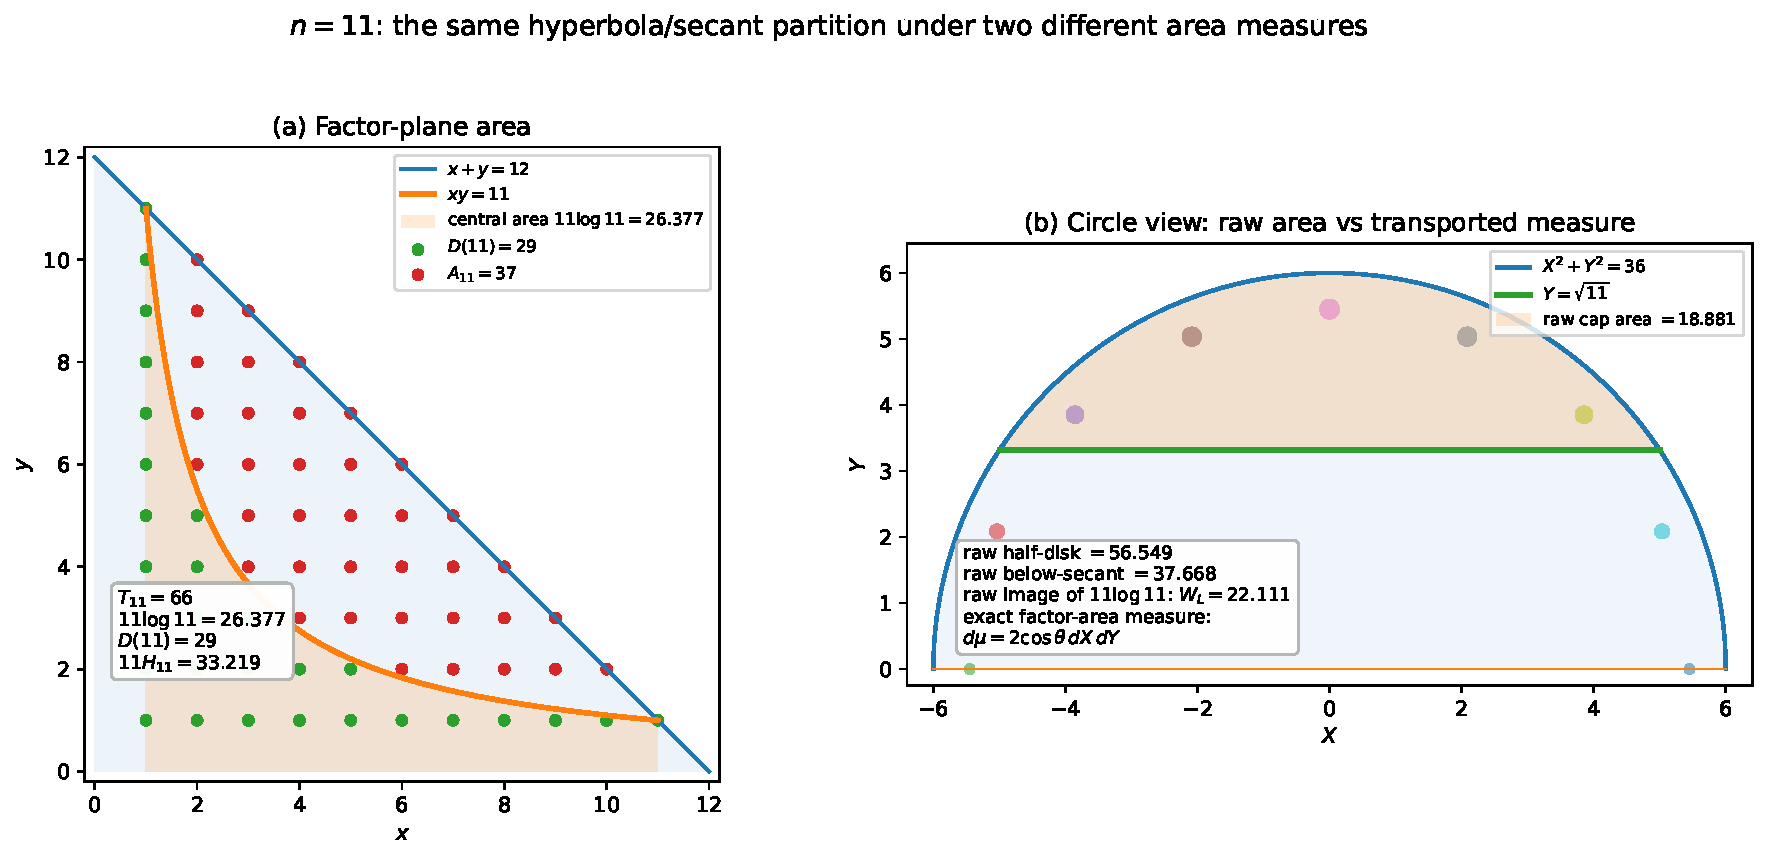
\includegraphics[width=\textwidth]{fig_area_measure_11_2panel.pdf}
\caption{The $n=11$ hyperbola/secant partition under two area measures. Left: the factor-plane triangle and the classical $xy=11$ boundary, with the continuous $11\log11$ region and the discrete $D(11)$/$A_{11}$ partition shown together. Right: the same continuous boundary is the secant $Y=\sqrt{11}$ of the radius-$6$ half-disk. Raw Euclidean circle area and transported factor-plane area are distinct: the exact factor-area measure in the circle view is $d\mu=2\cos\theta\,dX\,dY$.}
\label{fig:area11}
\end{figure}

\section{Conclusion}
The factor-plane triangle, the flat circle view, and the Euclidean cone surface carry three distinct but exactly related area measures. The first change of variables is nonuniform and is governed by $T/(2Y)$; the second is the constant factor $\sqrt2$. Constant-product hyperbolas become secants, and the complete shell partition has closed formulas in both coordinate systems. In product-ratio variables the same transformation sends logarithmic rapidity $s$ to ordinary circle angle $\theta$ through $d\theta=\operatorname{sech}s\,ds$, providing an exact logarithmic-to-circular compactification. The factor-plane area measure itself is recovered in circle coordinates by the canonical weight $2\cos\theta=2\operatorname{sech}s$. This weighted measure, rather than any global constant normalization, is the exact bridge needed for comparing factor-plane areas with their circular images.

\begin{thebibliography}{9}
\bibitem{Ebert2026Table} J.~Ebert, \emph{The Cutting Plane: Every Line Through the Multiplication Table Is a Conic Section}, 2026.
\bibitem{Ebert2026Semiclassical} J.~Ebert, \emph{A Semiclassical Band-Area Correspondence for the AM--GM Cone}, research note, 2026.
\end{thebibliography}

\end{document}
